\documentclass[12pt,a4paper]{scrartcl}
\usepackage[utf8]{inputenc}
\usepackage[english,russian]{babel}
\usepackage{indentfirst}
\usepackage{misccorr}
\usepackage{graphicx}
\usepackage{amsmath}
\graphicspath{}
\author{Даря}
\DeclareGraphicsExtensions{.pdf,.png,.jpg}
\begin{document}
\begin{flushright}
  Павлова Дарья\\
  19ПИ-1\\
  1.12.20\\
\end{flushright}

\section{Установка и настройка}
\textnumero \textbf{1. Samba}
\\[5pt]
\begin{center}
 sudo apt install samba
\end{center}
+ соглашаемся на установку всех пакетов
\\[5pt]
Создаём резервную копию конфигурационного файла. Если что-то пойдет не так, то файл можно будет восстановить из копии
\begin{center}
sudo cp /etc/samba/smb.conf /etc/samba/smb-b.conf
\end{center}
Создадим папку для шэринга и заполняем её чем-нибудь (у меня это файл cat1)
\begin{center}
mkdir cats\_photos
\end{center}
Открываем конфигурационный файл 
\begin{center}
sudo gedit /etc/samba/smb.conf 
\end{center}
-перейдем в конец файла и введем следующие строчки:
\\[5pt]
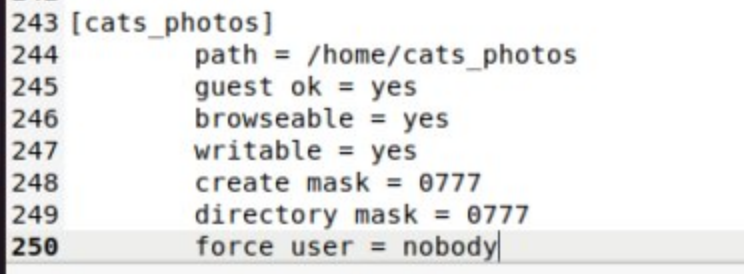
\includegraphics[scale=10, width=10cm]{f1}
\\[5pt]
Перезапускаем самбу
\\[5pt]
\begin{center}
sudo service smbd restart
\end{center}
\textnumero \textbf{2. nginx} \\[5pt]
\begin{center}
sudo apt install nginx
\end{center}
+ соглашаемся на установку всех пакетов \\[5pt]
делаем бэкаб конфигов \\[5pt]
\begin{center}
sudo cp /etc/nginx/sites-available/default /etc/nginx/sites-available/default-b
\end{center}
Изменяем конфигурацию \\
\begin{center}
sudo gedit /etc/nginx/sites-available/default
\end{center}
записываем в файлик данные строчки 
\\[5pt]
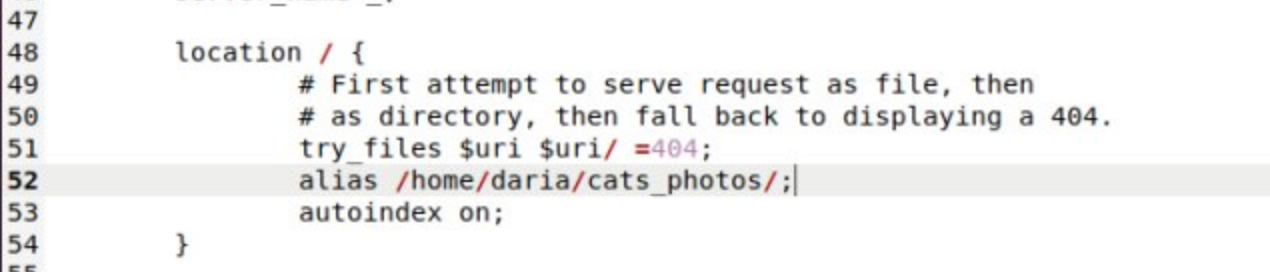
\includegraphics[scale=10, width=15cm]{f2}
\\[5pt]
\section{Настройка сети}
Настраиваем режим сетевого подключения в виртуальной машине
\\[5pt]
host-only означает, что наш ip будет доступен только на той машине, на котором запущена виртуальная машина
\\[5pt]
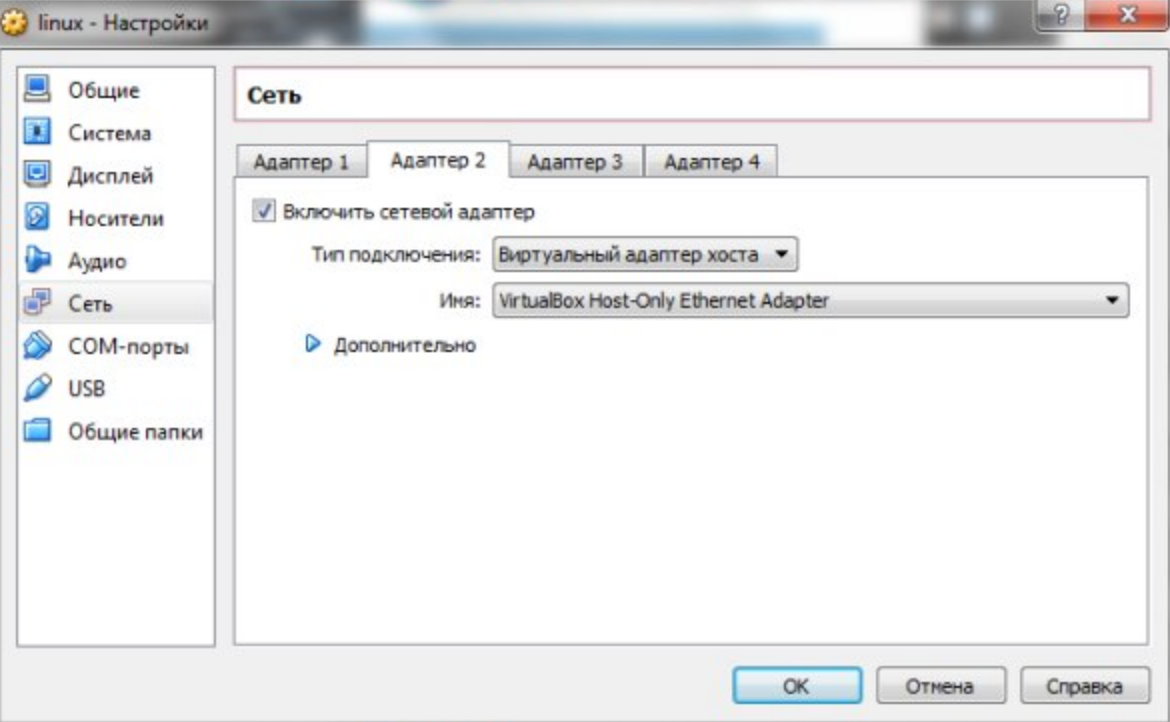
\includegraphics[scale=10, width=15cm]{f3}
\\[5pt]
узнаем ip
\\[5pt]
\begin{center}
sudo apt install net-tools
\end{center}
\begin{center}
sudo ifconfig
\end{center}
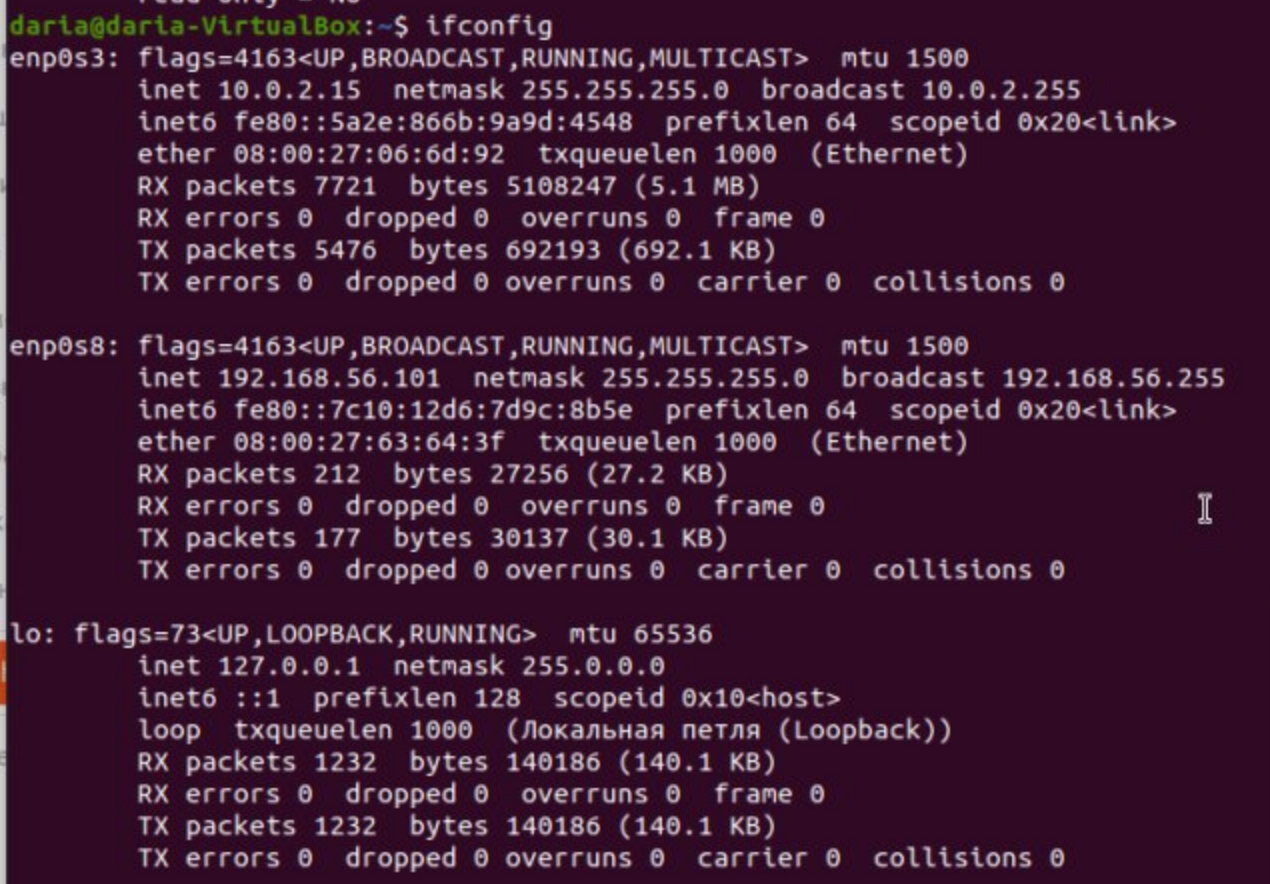
\includegraphics[scale=10, width=15cm]{f4} \\[5pt]
10.0.2.15 - локальный ip для самбы
\\[5pt]
192.168.56.101 - хостовой ip, заходим по нему через windows
\\[5pt]
\section{Просмотр папки}
\textnumero \textbf{1. Просмотр расшаренной папки nginx}\\
\textnumero \textbf{1.1 через linux:} \\[5pt]
http://localhost \\[5pt]
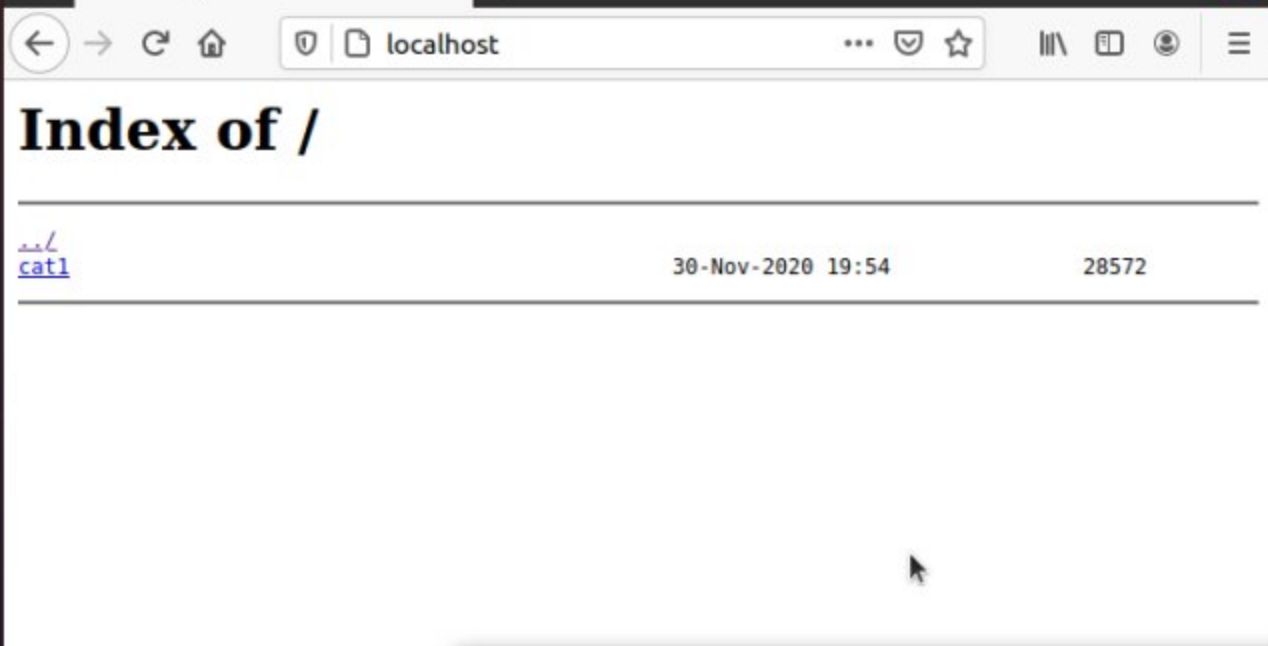
\includegraphics[scale=10, width=15cm]{f5} \\[5pt]
\textnumero \textbf{1.2 через windows:} \\[5pt] 
http://192.168.56.101 \\[5pt]
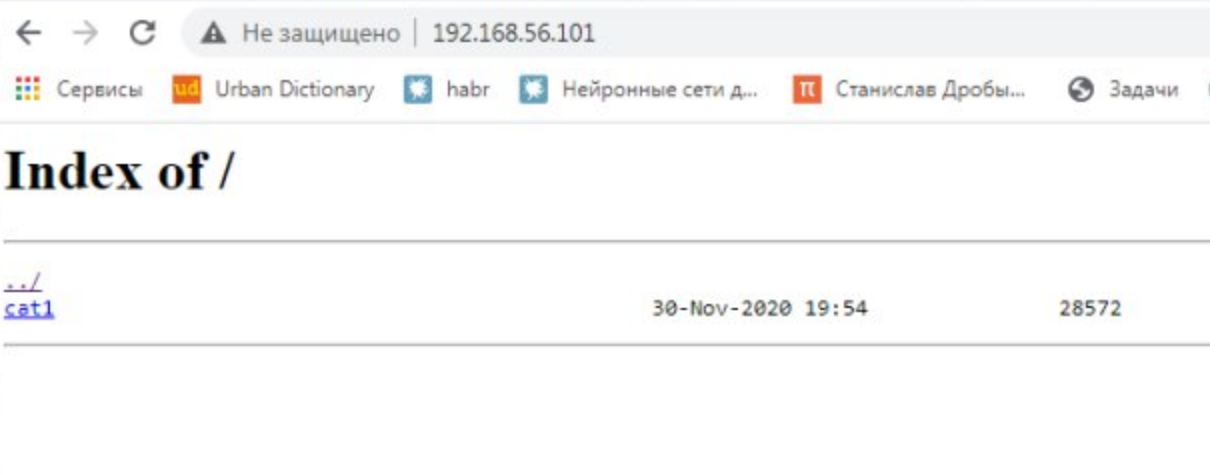
\includegraphics[scale=10, width=15cm]{f6} \\[5pt]
\textnumero \textbf{2. Просмотр расшаренной папки samba} \\[5pt]
\textnumero \textbf{2.1 через файловый менеджер linux:} \\[5pt]
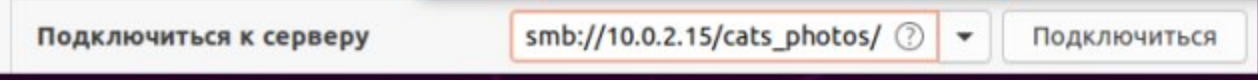
\includegraphics[scale=10, width=15cm]{f7} \\[5pt]
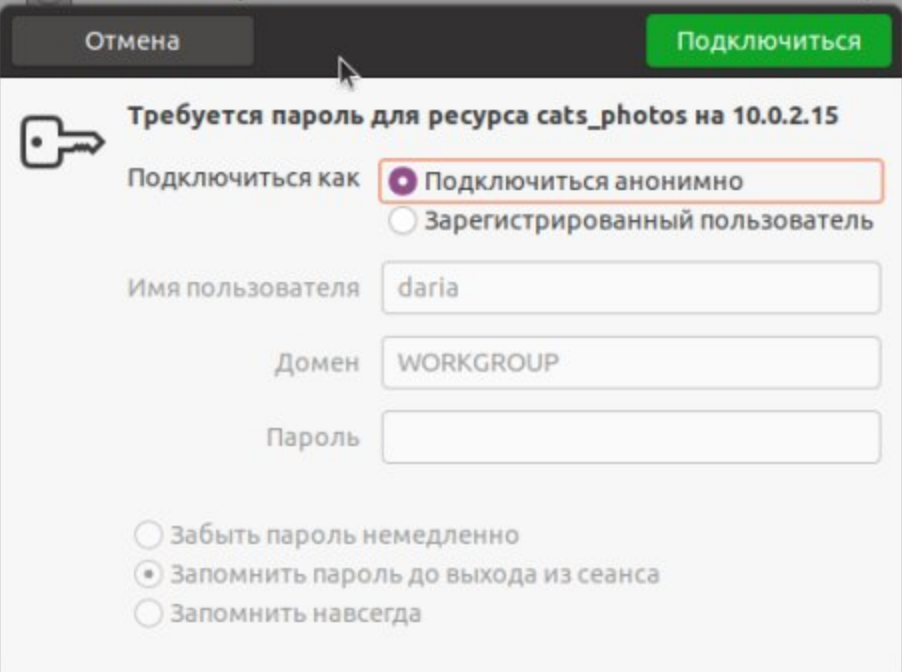
\includegraphics[scale=10, width=15cm]{f71} \\[5pt]
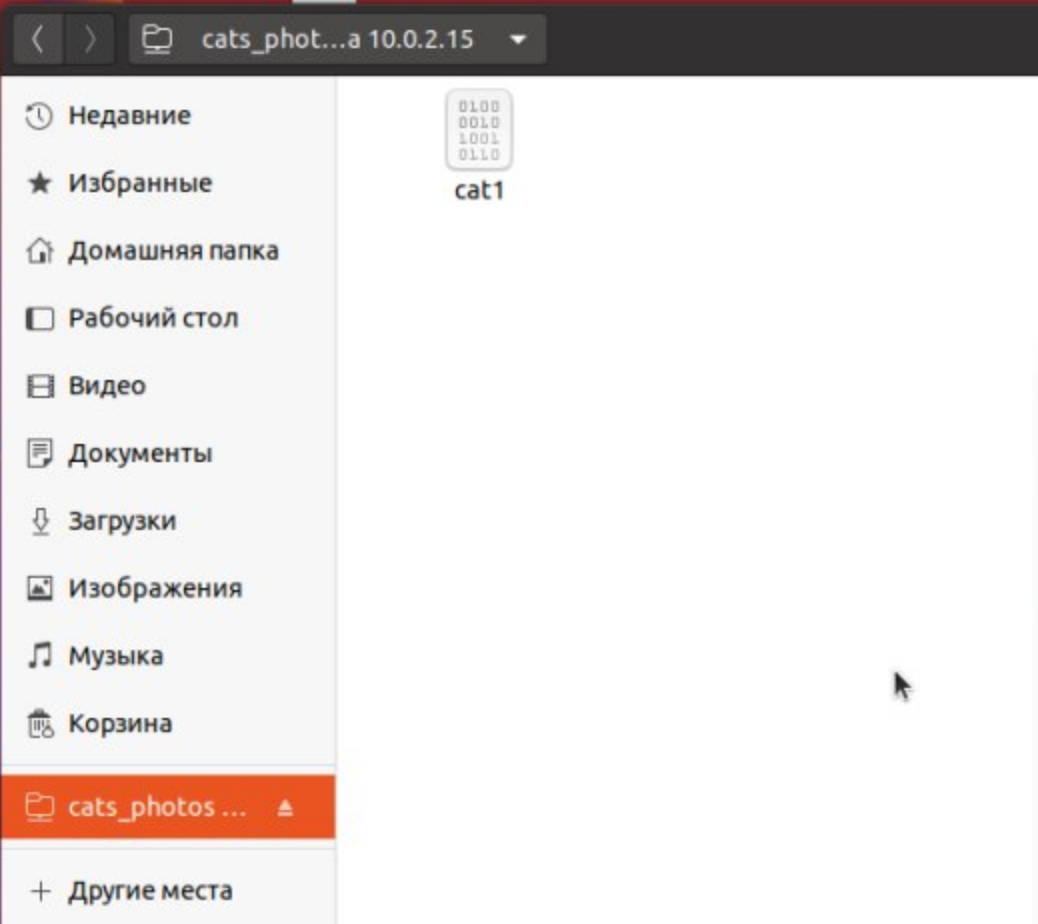
\includegraphics[scale=10, width=15cm]{f8} \\[5pt]
\textnumero \textbf{2.2 через файловый менеджер windows} \\[5pt]
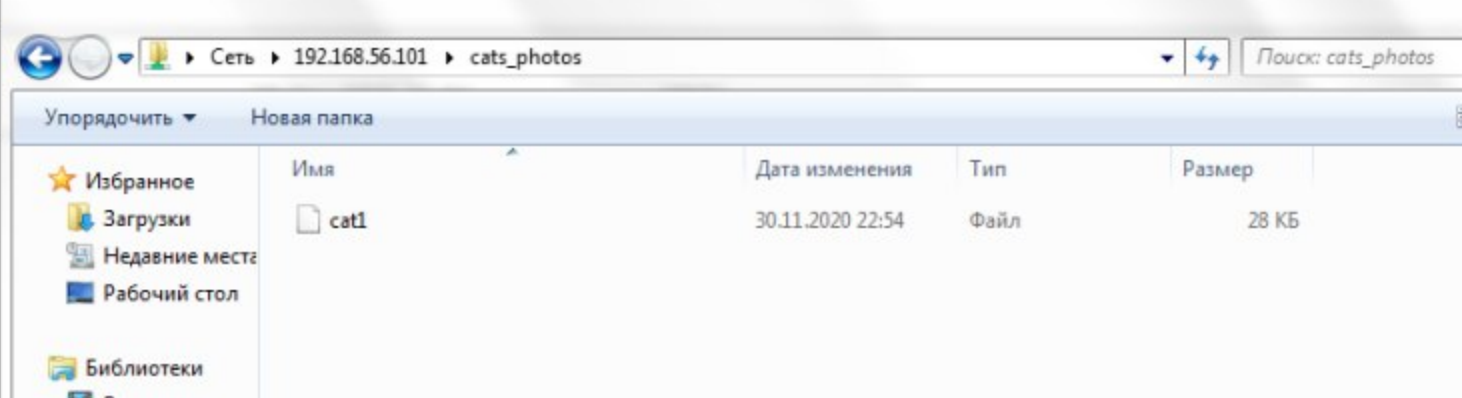
\includegraphics[scale=10, width=15cm]{f9}
\section{Усложнялка} 
\textnumero \textbf{1. Создание раздела}\\[5pt]
Создаём файл размером 100мб с помощью dd и форматируем с помощью mkfs.ext4 \\[5pt]
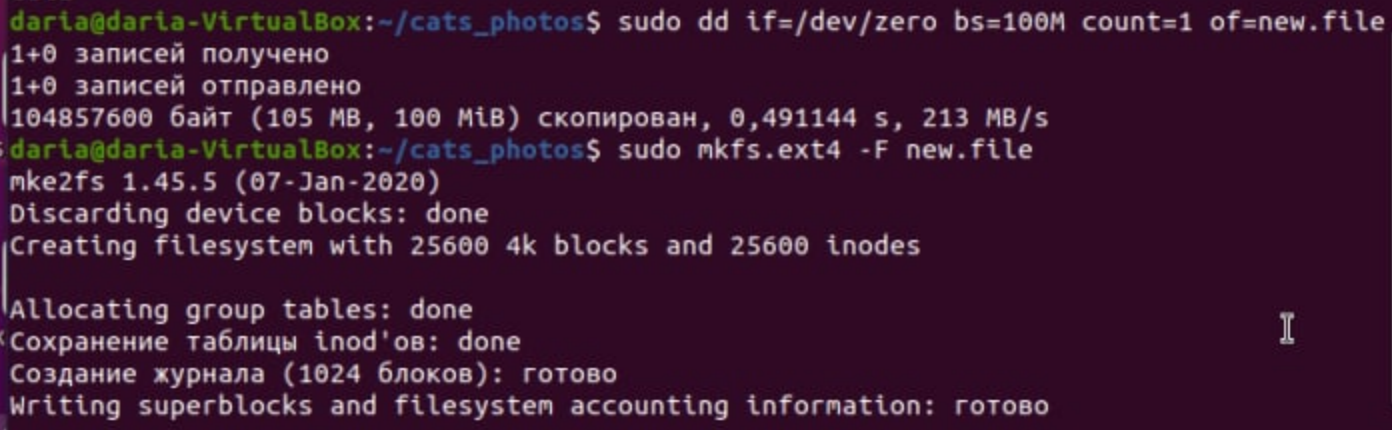
\includegraphics[scale=10, width=15cm]{f10} \\[5pt]
Монтируем файл в пустую папку \\[5pt]
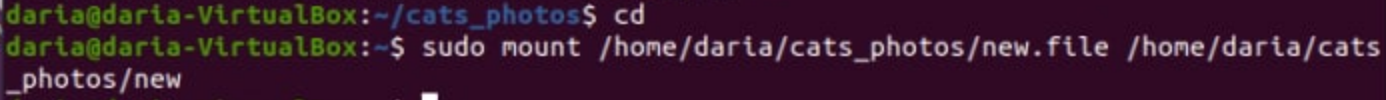
\includegraphics[scale=10, width=15cm]{f11} \\[5pt]
Раздаём права на папку всем пользователям, чтобы в неё можно было что-то положить
\begin{center}
sudo chmod -R 777 /home/daria/cats\_photos/new
\end{center}
\textnumero \textbf{2. Просмотр} \\[5pt]
\textnumero \textbf{2.1 Samba} \\[5pt]
Изменяем конфигурацию в smb.conf \\[5pt]
\begin{center}
sudo gedit /etc/samba/smb.conf 
\end{center}
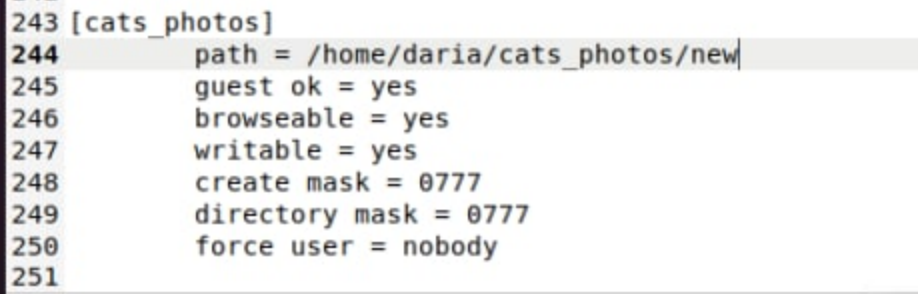
\includegraphics[scale=10, width=15cm]{f12}\\
Перезапускаем сервис \\[5pt]
\begin{center}
sudo service smbd restart
\end{center}
Получаем папку через файловый менеджер \\[5pt]
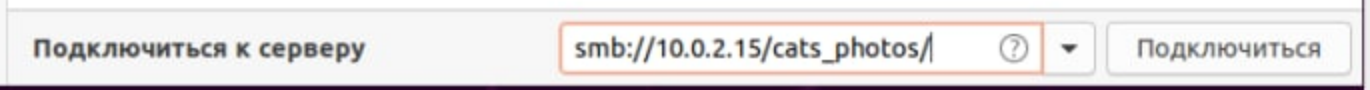
\includegraphics[scale=10, width=15cm]{f13} \\[5pt]
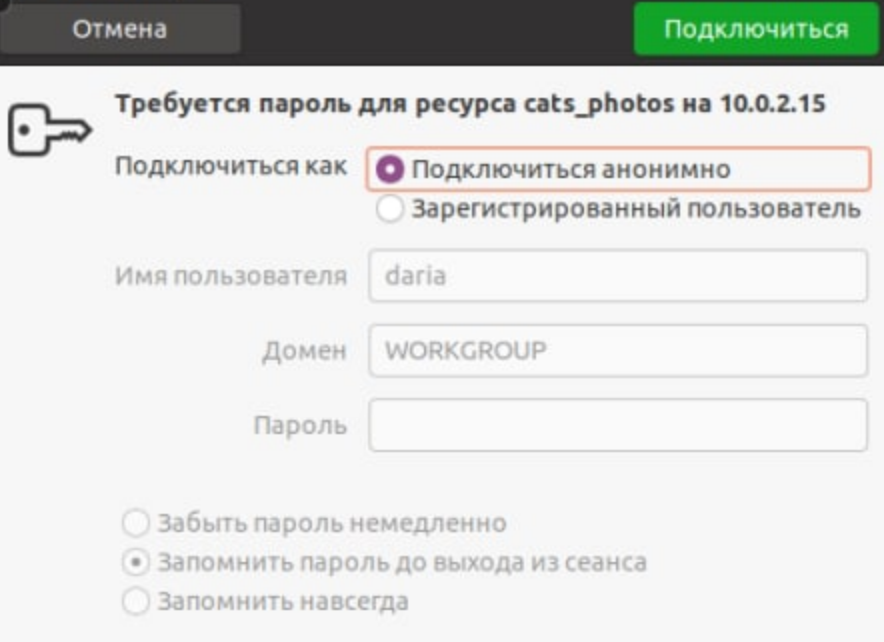
\includegraphics[scale=10, width=15cm]{f131} \\[5pt]
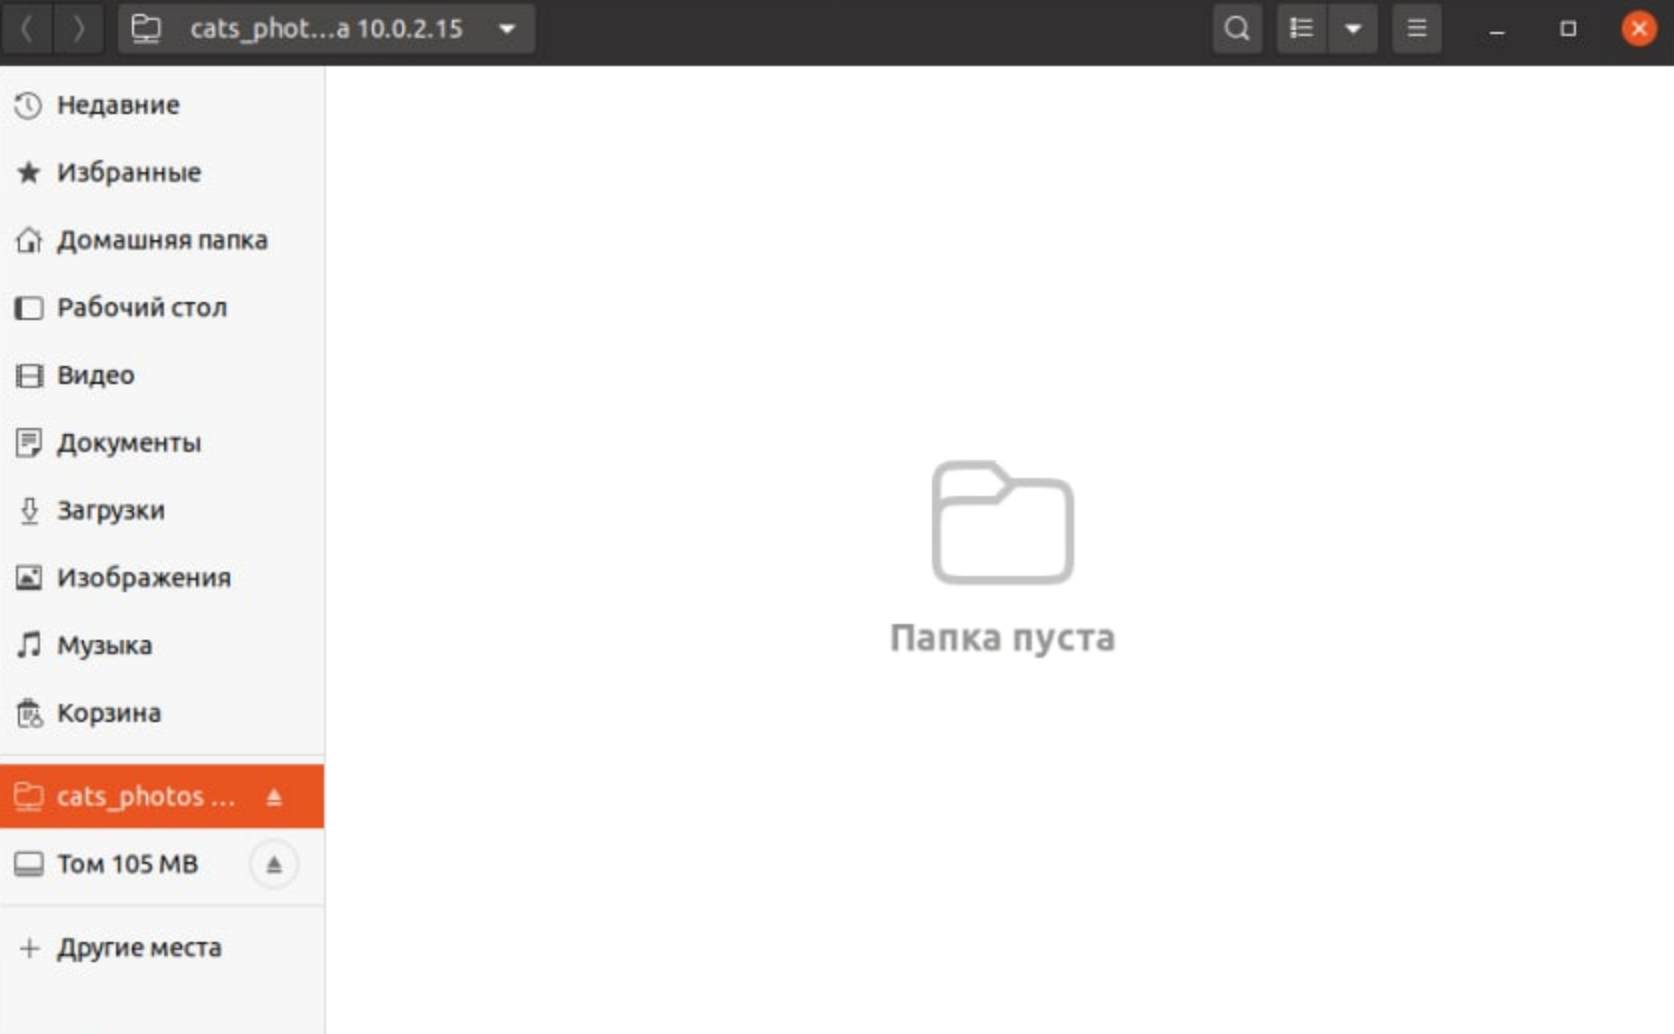
\includegraphics[scale=10, width=15cm]{f132} \\[5pt]
Просматриваем папку на windows \\[5pt]
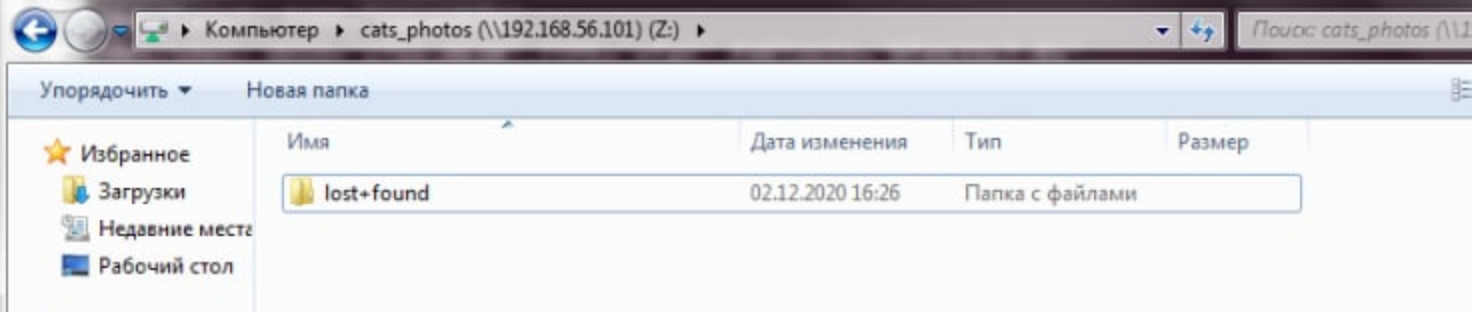
\includegraphics[scale=10, width=15cm]{f14} \\[5pt]
\textnumero \textbf{2.2 Nginx} \\[5pt]
Настраиваем конфигурацию
\begin{center}
sudo gedit /etc/nginx/sites-available/default
\end{center}
В файл дописываем нашу новую директорию  \\[5pt]
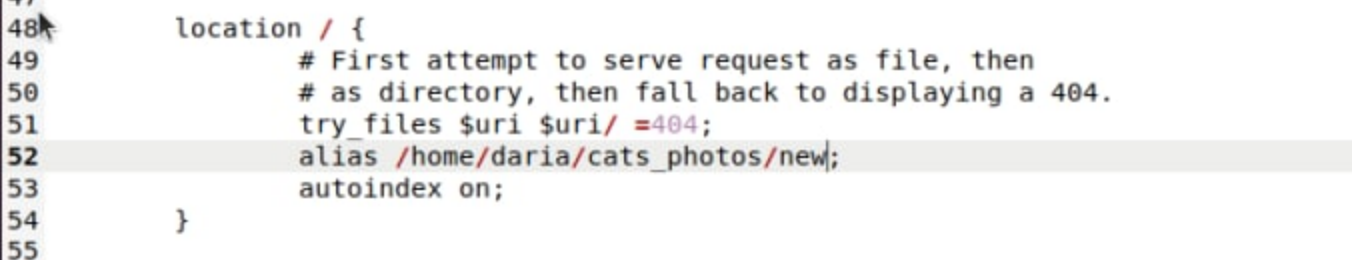
\includegraphics[scale=10, width=15cm]{f15} \\[15pt]
Перезапускаем сервисы
\begin{center}
sudo service nginx restart
\end{center}
Получаем папку через http://localhost на linux \\[15pt]
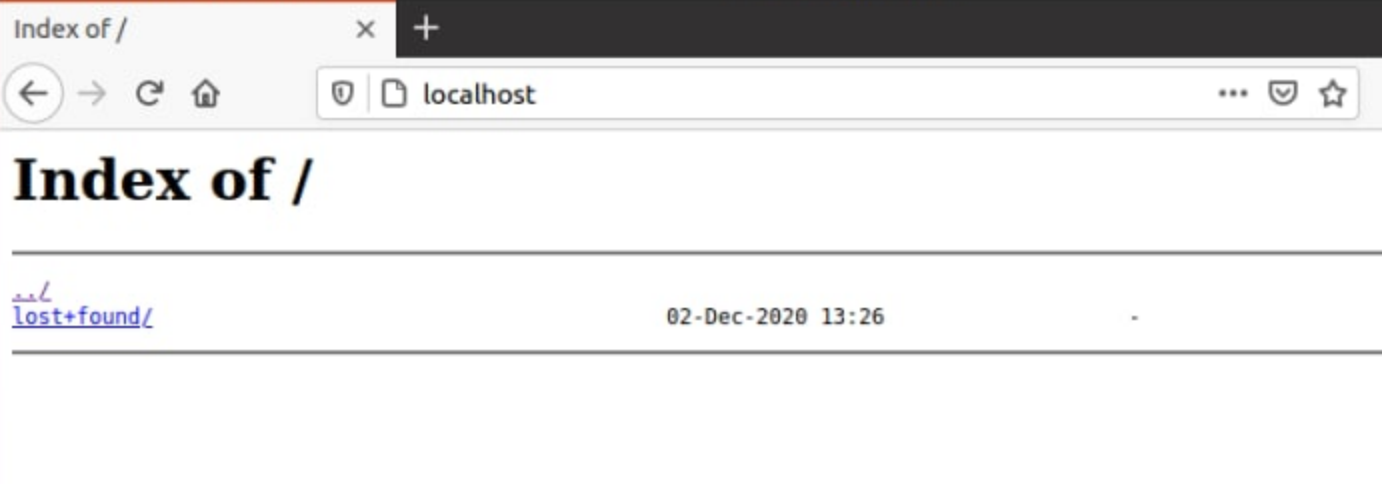
\includegraphics[scale=10, width=15cm]{f16} \\[15pt]
Получаем папку через http://192.168.56.101 на windows  \\[15pt]
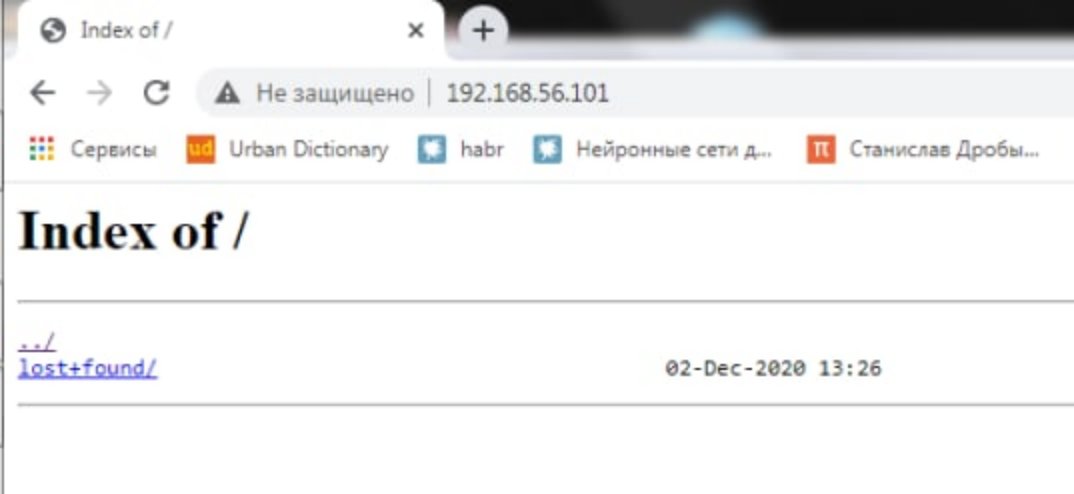
\includegraphics[scale=10, width=15cm]{f17} \\[15pt]
\textnumero \textbf{3. Backups:} \\[15pt]
Открываем cron:
\begin{center}
sudo crontab -e
\end{center}
Записываем в крон следующие строчки \\[15pt]

00 0 1 Jan * *  root tar -czf /root/backups/bs.tar.gz /home/daria/cats\_photos/new.file - для бэкапа на каждый новый год \\[15pt]

00 0 13 * Fri * root tar -czf /root/backups/bs.tar.gz /home/daria/cats\_photos/new.file - для бэкапа на каждую пятницу 13

\end{document}